% Report content: b813f47d-864f-4422-92c8-e6f81b30efae
% Describe the problem you are solving.  This does not need to be very in depth but should provide the reader with any 
% information they need in order to understand what you are doing.
% You can cite references but we are after *your* statement of the problem not a copy paste from elsewhere.

% Describe your implementation.   This should not be a copy of your source code but should have enough detail to allow the 
% reader to understand how your program works. You should definitely describe any data structures you have employed as well as any 
% optimisations you have attempted.

% Describe how you know that it works.  This applies to both the correctness and performance. "I tested it with a few cases" 
% would be a low quality answer. How many test cases? Why those cases?  If you used optimisations, did they work? (Both in 
% terms of preserving correctness and actually improving performance).

% Description of performance. (Note that this is a bit more flexible than what is listed in the ECP).  What can you say about the performance 
% of your implementation? How does the run time vary with different inputs? You can also include content about 
% profiling or internal timing analysis you have done here.
%%
\documentclass[preprint,12pt]{elsarticle}

%% Use the option review to obtain double line spacing
%% \documentclass[preprint,review,12pt]{elsarticle}

%% Use the options 1p,twocolumn; 3p; 3p,twocolumn; 5p; or 5p,twocolumn
%% for a journal layout:
%% \documentclass[final,1p,times]{elsarticle}
%% \documentclass[final,1p,times,twocolumn]{elsarticle}
%% \documentclass[final,3p,times]{elsarticle}
%% \documentclass[final,3p,times,twocolumn]{elsarticle}
%% \documentclass[final,5p,times]{elsarticle}
%% \documentclass[final,5p,times,twocolumn]{elsarticle}

%% The graphicx package provides the includegraphics command.
\usepackage{graphicx}
%% The amssymb package provides various useful mathematical symbols
% \usepackage[demo]{graphicx}
\usepackage{bm,amssymb,amsmath,amsfonts,mathrsfs,stmaryrd,amssymb,mathtools,subfig,caption,float,minted,longtable,url,hyperref}
\usepackage[linesnumbered,lined,boxed,vlined,ruled]{algorithm2e}
\usepackage[margin=1.05in]{geometry}
\renewcommand{\baselinestretch}{1.3}
%% The amsthm package provides extended theorem environments
%% \usepackage{amsthm}

%% The lineno packages adds line numbers. Start line numbering with
%% \begin{linenumbers}, end it with \end{linenumbers}. Or switch it on
%% for the whole article with \linenumbers after \end{frontmatter}.
\usepackage{lineno}

\newtheorem{theorem}{Theorem}[section]
\newtheorem{corollary}{Corollary}[theorem]
\newtheorem{lemma}[theorem]{Lemma}

\newcommand{\norm}[1]{\left\lVert#1\right\rVert}
%% natbib.sty is loaded by default. However, natbib options can be
%% provided with \biboptions{...} command. Following options are
%% valid:

%%   round  -  round parentheses are used (default)
%%   square -  square brackets are used   [option]
%%   curly  -  curly braces are used      {option}
%%   angle  -  angle brackets are used    <option>
%%   semicolon  -  multiple citations separated by semi-colon
%%   colon  - same as semicolon, an earlier confusion
%%   comma  -  separated by comma
%%   numbers-  selects numerical citations
%%   super  -  numerical citations as superscripts
%%   sort   -  sorts multiple citations according to order in ref. list
%%   sort&compress   -  like sort, but also compresses numerical citations
%%   compress - compresses without sorting
%%
%% \biboptions{comma,round}

% \biboptions{}

\journal{Journal Name}

\begin{document}

\begin{frontmatter}

%% Title, authors and addresses

\title{STAT4402 Tutorial}

\author{Michael Ciccotosto-Camp}

\address{University of Queensland}

% \begin{abstract}
% Programs which find the Longest Common Substring (LCS) are employed many areas of scientific endeavour; most notably in bio-informatics and computer science. In this report a Dynamic bottom-up algorithm is implemented (in \texttt{main.c}) to find the LCS of two strings in the {\it C} programming language. The most effective optimizations found to decrease run-time included using 1D matrices, conservative subroutine calling, loop-interchanging and loop-unrolling
% \end{abstract}

\end{frontmatter}

\section{Introduction}
Most computational work done within science is impractical to perform on commercial laptops and desktops, typically due to the extremely high memory and processing demands. Hence, almost every university and industry has its own high-performance computer to carry out such strenuous problems. A lot of research within the realm of Machine Learning benefits from access to high performance machinery as most of them require matrix computation (which can be efficiently carried out on GPU clusters) and can be processed in parallel.\\[1\baselineskip]
In this tutorial we will revisit three models covered in the first few weeks of lectures, these being the k-NN classifier, the perceptron and SDG linear regressor. The serial implementations for theses algorithms maybe become fairly inefficient large data sets, so we shall look at some ways in which these two methods can be decomposed and parallelised.
\newpage

\section{Parallel KNN}
% See ESLII page 33
% See Dirk page
The $k^{th}$ Nearest-Neighbor (k-NN) methods uses observations from a training set $T$ to find its closest neighbours in feature space to a given an unknown sample $\bm{x}$ a prediction value $\overline{y}$ \cite{HastieTrevor2009EoSL}. The prediction for the k-NN classifier is usually calculated as an average or consensus vote, that is
\[
    \overline{y} \left( \bm{x} \right) = \sum_{\bm{x}_{i} \in N_{k} (\bm{x})} y_{i}
\]
The notion of 'closest' implies the use of some sort of metric. More often than not, feature vectors belong to some subset $\mathbb{R}^{n}$, allowing us to apply commonly used metrics to define distance between vectors in our feature space. For our purposes, we shall use the Euclidean norm as a measurement of determining how close two feature values are to each other. The Euclidean norm is simply defined as
\[
    d \left( \bm{x}, \bm{y} \right) = \left( \sum_{i=1}^{n} \left( x_{i} - y_{i} \right)^{2} \right)^{\frac{1}{2}}.
\]
Other metrics such as Manhatten norm or hamming distance for discrete feature spaces \cite{HastieTrevor2009EoSL}. When a unknown sample $\bm{x}$ is to be classified, a k-NN classifier computes the distance between $\bm{x}$ and the other points within the training set $T$. The training data is then sorted by distance and the $k^{th}$ closests training samples are then used to predict $\bm{x}$. A simple K-NN algorithm is presented in algorithm \ref{alg:serial-k-NN}.
\begin{algorithm}[ht!!!]
\caption{Serial k-NN}
\label{alg:serial-k-NN}
\SetAlgoLined
    \SetKwInOut{Input}{input}\SetKwInOut{Output}{output}
    
    \Input{Training data $T$, an unlabelled sample $\bm{x}$ and a value $k$}
    \Output{Predicted class $\overline{y} \left( \bm{x} \right)$}
    \BlankLine
    Computes distance $d \left( \bm{x}, \bm{x}_{t_i} \right)$ for each $\bm{x}_{t_i} \in T$\;
    $N_{k} (\bm{x}) \gets$ the $k^{th}$ closest $\bm{x}_{t_i}$ determined by $d \left( \bm{x}, \bm{x}_{t_i} \right)$\;
    $\overline{y} \left( \bm{x} \right) \gets \sum_{\bm{x}_{i} \in N_{k} (\bm{x})} y_{i}$\;
    \KwResult{$\overline{y} \left( \bm{x} \right)$}
    \BlankLine
\end{algorithm}
While this method is simple, computing the distance between $\bm{x}$ and each $\bm{x}_{t_i} \in T$ can incur a large time overhead, especially for large training sets. In order to parallize this algorithm, one important observation is that computing the distances $d \left( \bm{x}, \bm{x}_{t_i} \right)$ and $d \left( \bm{x}, \bm{x}_{t_j} \right)$ where $\bm{x}_{t_i}, \bm{x}_{t_j} \in T$ and $i \neq j$ allowing us to carry out these computations on separate processes. Liang et al. (2010) takes advantage of this independence by splitting up the training examples into $p$ partitions and send these partitions to slave processes to compute the distances between feature vectors in our training example and a unknown sample $\bm{x}$. The $k^{th}$ closet training examples are found within individual slaves and are collected within the master process. Combining the $k^{th}$ closet acquired by each process locally, the master process then sorts the reduced list of training vectors to find the global $k^{th}$ closet training examples \cite{ShenshenLiang2010Daeo}. Pseudo code for parallel KNN is shown in \ref{alg:parallel-k-NN}.
\begin{algorithm}[h!!!]
\caption{Parallel k-NN}
\label{alg:parallel-k-NN}
\SetAlgoLined
    \SetKwInOut{Input}{input}\SetKwInOut{Output}{output}
    \Input{Training data $T$, an unlabelled sample $\bm{x}$, a value $k$ and the number of processes to perform the algorithm $p$}
    \Output{Predicted class $\overline{y} \left( \bm{x} \right)$}
    \BlankLine
    $\left\lbrace T_{1} , T_{2}, \ldots , T_{p} \right\rbrace \gets$ an equal partition of $T$\;
    \For{$T_{i} \in \left\lbrace T_{1} , T_{2}, \ldots , T_{p} \right\rbrace$ {\bf concurrently}}{
        $N_{k_i} (\bm{x}) \gets$ the $k^{th}$ nearest neighbors from $T_{i}$\;
    }
    $N_{k} (\bm{x}) \gets$ the $k^{th}$ closest neighbors from $N_{k_1} (\bm{x}), N_{k_2} (\bm{x}), \ldots N_{k_p} (\bm{x})$\;
    $\overline{y} \left( \bm{x} \right) \gets \sum_{\bm{x}_{i} \in N_{k} (\bm{x})} y_{i}$\;
    \KwResult{$\overline{y} \left( \bm{x} \right)$}
    \BlankLine
\end{algorithm}

This algorithm is shown pictorially below\\
\renewcommand{\labelenumi}{\textbf{Step \arabic{enumi})}}
\begin{enumerate}
    \item Partition the data and send partitions to processes \(P_{1}, P_{2}, P_{3}, P_{4}\)
    \begin{figure}[H]
        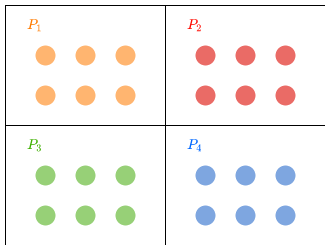
\includegraphics[scale=0.8]{img/STAT4402_tut_KNN_1_no_cap.png}
        \centering
    \end{figure}
    
    \item Determine the closest samples within each process
    \begin{figure}[H]
        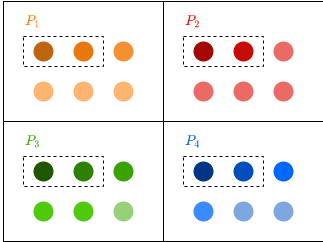
\includegraphics[scale=0.8]{img/STAT4402_tut_KNN_2_no_cap.png}
        \centering
    \end{figure}
    
    \item Collect the \(k^{th}\) closest samples and order them in the master node get the global
\(k^{th}\) closest samples
    \begin{figure}[H]
        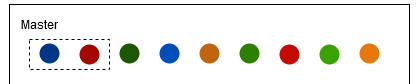
\includegraphics[scale=0.7]{img/STAT4402_tut_KNN_3_no_cap.png}
        \centering
    \end{figure}
\end{enumerate}
\newpage

\section{Parallel Multiclass Perceptron}

Similar to a definition is class the perception is an algorithm that uses an affine function as a threshold boundary to classify real valued feature vectors. The output of a perceptron is simply given as
\[
    f(\mathbf{x})=\left\{\begin{array}{ll}
    1 & \text { if } \mathbf{w} \cdot \mathbf{x}+b>0 \\
    0 & \text { otherwise }
    \end{array}\right.
\]
where $\bm{w} \in \mathbb{R}^{m}$ with $b$ acting as a bias. A simple generalisation we can make to the perceptron is to allow it to predict more than just two classes. This is known as the {\it multiclass perceptron} \cite{HastieTrevor2009EoSL}. A feature representation function maps a feature vector and its correspond label to a real valued vector. This output vector is then dot-producted with  a weight vector $\bm{w}$, similar to the 'two-class' perceptron. The prediction value of an unknown feature vector for the multi-class perceptron can be computed as
\[
    \overline{y} \left( \bm{x} \right) = \underset{y}{\arg \min } \; \bm{w} \cdot f(\bm{x}, y)
\]
The iterative procedure to create our weight vector from the training set is also similar, although this time if we make an incorrect prediction we move the weight vector in the direction of $f(\bm{x}, y) - f(\bm{x}, \overline{y})$ \cite{HastieTrevor2009EoSL}. The algorithm for the serial multi-class perceptron is shown in Algorithm \ref{alg:serial-perceptron}. Note, for the sake of simplicity a learning rate parameter has been omitted within the training algorithm.
\begin{algorithm}[ht!!!]
    \caption{Serial Multiclass Perceptron}
    \label{alg:serial-perceptron}
    \SetAlgoLined
    \SetKwInOut{Input}{input}\SetKwInOut{Output}{output}
    \Input{Training data $T$, an initial weight vector $\bm{w}^{(0)}$}
    \Output{Updated weight vector}
    \BlankLine
    $k \gets 0$;
    
    \While{until convergence}{
    
        \For{$\left( \bm{x}_{i}, y_{i} \right) \in T$}{
        
            $\overline{y} \gets \underset{y}{\arg \min } \; \bm{w}^{(k)} \cdot f(\bm{x}, y)$\;
            $k \gets k+1$\;
            
            \uIf{$\overline{y} \neq y$}{
                $\bm{w}^{(k+1)} \gets \bm{w}^{(k)} + f(\bm{x}, y) - f(\bm{x}, \overline{y})$\;
            }
        }
    }
    \KwResult{$\bm{w}^{(k)}$}
    \BlankLine
\end{algorithm}
One obvious way to parallise Algorithm \ref{alg:serial-perceptron} is to split the training set $T$ into $p$ partitions. One can then train an initial weight on each of these partitions independently on the $p$ processes and then take a weighted mixture of the weights from each of the different processes \cite{10.5555/1857999.1858068}. The mixture coefficents will be given as the vector $\bm{\mu}$ where $\mu_{i} \geq 0$ and $\sum_{i} \mu_{i} = 1$. Pseudo-code for this naive parallel multi-class perceptron is shown in Algorithm \ref{alg:serial-perceptron}.
\begin{algorithm}[ht!!!]
    \caption{Naive Parallel Multiclass Perceptron}
    \label{alg:naive-parallel-perceptron}
    \SetAlgoLined
    \SetKwInOut{Input}{input}\SetKwInOut{Output}{output}
    \Input{Training data $T$, an initial weight vector $\bm{w}^{(0)}$}
    \Output{Updated weight vector}
    \BlankLine
    $k \gets 0$\;
    
    $\left\lbrace T_{1} , T_{2}, \ldots , T_{p} \right\rbrace \gets$ an equal partition of $T$\;
    \For{$T_{i} \in \left\lbrace T_{1} , T_{2}, \ldots , T_{p} \right\rbrace$ {\bf concurrently}}{
        $\bm{w}^{(i)} = \operatorname{Serial Multiclass Perceptron} \left( T, \bm{w}^{(0)} \right)$\;
    }
    
    $\bm{w} = \sum_{i} \mu_{i} \bm{w}^{(i)}$\;
    
    \KwResult{$\bm{w}$}
    \BlankLine
\end{algorithm}
While Algorithm \ref{alg:naive-parallel-perceptron} is easy to understand and makes effective use of parallel resources without incurring too much over-head in inter-process communication, it has one large shortcoming. Even for linearly separable data sets $T$, algorithm \ref{alg:naive-parallel-perceptron} does not always converge to a separating hyperplane. In fact in Question {\bf 2b} you will be asked to provide a linearly separable data set for which algorithm \ref{alg:naive-parallel-perceptron} will not converge. To salvage this parallel algorithm we can make sure each process is communicating there results more often before finalizing $\bm{w}$. That is we can collect weights from processors after each single epoch, mix these the weights together and then redistribute this new weight vector to our processes again for a new epoch \cite{10.5555/1857999.1858068}. This new iterative parameter mixing idea is shown in Algorithm \ref{alg:parallel-perceptron}.
\begin{algorithm}[ht!!!]
    \caption{Parallel Multiclass Perceptron}
    \label{alg:parallel-perceptron}
    \SetAlgoLined
    \SetKwInOut{Input}{input}\SetKwInOut{Output}{output}
    \Input{Training data $T$, an initial weight vector $\bm{w}^{(0)}$}
    \Output{Updated weight vector}
    \BlankLine
    $\bm{w} \gets \bm{w}^{(0)}$\;
    \For{$n \in \left\{ 1,2, \ldots , N \right\}$}{
    \For{$T_{i} \in \left\lbrace T_{1} , T_{2}, \ldots , T_{p} \right\rbrace$ {\bf concurrently}}{
            $\bm{w}^{(i,n)} = \operatorname{One Perceptron Epoch} \left( T_{i}, \bm{w} \right)$\;
        }
        $\bm{w} \gets \sum_{i} \mu_{i} \bm{w}^{(i,n)}$\;
    }
    \KwResult{$\bm{w}$}
    \BlankLine
\end{algorithm}
\begin{algorithm}[ht!!!]
    \caption{One Perceptron Epoch}
    \label{alg:one-perceptron-epoch}
    \SetAlgoLined
    \SetKwInOut{Input}{input}\SetKwInOut{Output}{output}
    \Input{Training data $T_{i}$, an initial weight vector $\bm{w}^{(0)}$}
    \Output{Updated weight vector}
    \BlankLine
    $k \gets 0$\;
    $\bm{w} \gets \bm{w}^{(0)}$\;
    \For{$\left( \bm{x}_{i}, y_{i} \right) \in T_{i}$}{
        
        $\overline{y} \gets \underset{y}{\arg \max } \; \bm{w}^{(k)} \cdot f(\bm{x}_{i}, y_{i})$\;
        
        \uIf{$\overline{y} \neq y$}{
            $\bm{w}^{(k+1)} \gets \bm{w}^{(k)} + f(\bm{x}_{i}, y_{i}) - f(\bm{x}_{i}, \overline{y})$\;
            $k \gets k+1$\;
        }
    }
    \KwResult{$\bm{w}^{(k)}$}
    \BlankLine
\end{algorithm}
The obvious and main drawback of algorithm \ref{alg:parallel-perceptron} over \ref{alg:naive-parallel-perceptron} this that there is much more inter-process communication overhead in reducing $\bm{w}^{(i,n)}$ and sending new values of $\bm{w}$. However, we will see that algorithm \ref{alg:parallel-perceptron} will in fact always converge for linearly separable training sets. We can show this in the following theorem:
\newpage
{\bf Theorem: } {\it Assuming a training set $T$ is linearly separable by a margin $\lambda$, let $k_{i,n}$ be the number of mistakes that occur ed on partition $i$ of the training set during the $n^{th}$ epoch of training. For any $N$, when training a perception with fixed parameter mixing in Algorithm \ref{alg:parallel-perceptron}}. \cite{10.5555/1857999.1858068}
\[
    \sum_{n=1}^{N} \sum_{i=1}^{S} \mu_{i,n} k_{i,n} \leq \frac{R^{2}}{\lambda^2}
\]
Borrowing some notation from before, let $\bm{w}^{(i,n)}$ be the weight acquired on the $n^{th}$ epoch of training by process $i$ and let $\bm{w}^{([i,n]-k)}$ be the weight vector for $\text{process}-i$, $k$ iterations back. Let $\bm{w}^{(avg,n)}$ be the weighted mixture weight for the $n^{th}$ epoch, that is
\[
    \bm{w}^{(avg,n)} = \sum_{i=1}^{S} \mu_{i,n} \bm{w}^{(i,n)}
\]
we can easily enough show that
\begin{equation}
    \label{eqn:R1}
    \bm{u} \cdot \bm{w}^{(i,n)} \geq \bm{u} \cdot \bm{w}^{(avg,n-1)} + k_{i,n} \lambda \tag{R1}
\end{equation}
and
\begin{equation}
    \label{eqn:R2}
    \norm{\bm{w}^{(i,n)}}^2 \leq \norm{\bm{w}^{(avg,n-1)}}^2 + k_{i,n} R^2 \tag{R2}
\end{equation}
Using \ref{eqn:R1} and \ref{eqn:R2} we can inductively show the following results
\begin{equation}
    \label{eqn:H1}
    \bm{u} \cdot \bm{w}^{(avg,n)} \geq \sum_{n=1}^{N} \sum_{i=1}^{S} \mu_{i,n} k_{i,n} \lambda \tag{H1}
\end{equation}
and
\begin{equation}
    \label{eqn:H2}
    \norm{\bm{w}^{(i,n)}}^2 \leq \sum_{n=1}^{N} \sum_{i=1}^{S} \mu_{i,n} k_{i,n} R^2 \tag{H2}
\end{equation}
we can see that \ref{eqn:R1} implies $\norm{\bm{w}^{(i,n)}} \geq \sum_{n=1}^{N} \sum_{i=1}^{S} \mu_{i,n} k_{i,n} \lambda$ since $\bm{v} \cdot \bm{w} \leq \norm{\bm{u}} \norm{\bm{w}}$ (by the Cauchy Schwarz inequality) and $\norm{\bm{u}} = 1$. For the base case $\bm{w}^{(avg,1)}$, using \ref{eqn:R1} and the fact that $\bm{w}^{(avg,0)} = 0$ 
\begin{align*}
    \bm{u} \cdot \bm{w}^{(avg,1)} = \sum_{i=1}^{S} \mu_{i,1} \bm{u} \cdot \bm{w}^{(i,1)} \geq \sum_{i=1}^{S} \mu_{i,1}  k_{i,n} \lambda
\end{align*}
To show \ref{eqn:H2}, the base case can be written as
\begin{align*}
    \norm{\bm{w}^{(avg,1)}}^2 &= \norm{\sum_{i=1}^{S} \mu_{i,1}}^2 \bm{w}^{(i,1)} \\
    &\leq \sum_{i=1}^{S} \mu_{i,1} \norm{\bm{w}^{(i,1)}}^{2} \\
    &\leq \sum_{i=1}^{S} \mu_{i,1} k_{i,n} R^2
\end{align*}
This expression is found by first applying Jensen's inequality followed by \ref{eqn:R2} as well as the fact that $\norm{\bm{w}^{(avg,0)}}^2 = 0$. Now considering the $N^{th}$ case, $\norm{\bm{w}^{(avg,N)}}^2$
\begingroup
\allowdisplaybreaks
\begin{align*}
    \bm{u} \cdot \bm{w}^{(avg,N)} &= \sum_{i=1}^{S} \mu_{i,N} \left( \bm{u} \cdot \bm{w}^{(i,N)} \right) \\
    &\geq \sum_{i=1}^{S} \mu_{i,N} \left( \bm{u} \cdot \bm{w}^{(avg,N-1)} + k_{i,N} \lambda \right) \tag{Using \ref{eqn:H1}} \\
    &= \bm{u} \cdot \bm{w}^{(avg,N-1)} + \sum_{i=1}^{S} \mu_{i,N} k_{i,N} \lambda \\
    &\geq \left[\sum_{n=1}^{N-1} \sum_{i=1}^{S} \mu_{i, n} k_{i, n} \lambda\right]+\sum_{i=1}^{S} \mu_{i, N} k_{i, N} \\
    &= \sum_{n=1}^{N} \sum_{i=1}^{S} \mu_{i, n} k_{i, n} \lambda
\end{align*}
\endgroup
Which thusly proves \ref{eqn:H1}. To show the inductive case for \ref{eqn:H2} we have
\begingroup
\allowdisplaybreaks
\begin{align*}
    \left\|\mathbf{w}^{(\mathrm{avg}, N)}\right\|^{2} &\leq \sum_{i=1}^{S} \mu_{i, N}\left\|\mathbf{w}^{(i, N)}\right\|^{2} \\
    &\leq \sum_{i=1}^{S} \mu_{i, N}\left(\left\|\mathbf{w}^{(\mathrm{avg}, N-1)}\right\|^{2}+k_{i, N} R^{2}\right) \\
    &= \left\|\mathbf{w}^{(\mathrm{avg}, N-1)}\right\|^{2}+\sum_{i=1}^{S} \mu_{i, N} k_{i, N} R^{2} \\
    &\leq \left[\sum_{n=1}^{N-1} \sum_{i=1}^{S} \mu_{i, n} k_{i, n} R^{2}\right]+\sum_{i=1}^{S} \mu_{i, N} k_{i, N} R^{2} \\
    &= \sum_{n=1}^{N} \sum_{i=1}^{S} \mu_{i, n} k_{i, n} R^{2}
\end{align*}
\endgroup
This shows \ref{eqn:H2}. Combining the results of \ref{eqn:H1} and \ref{eqn:H2} as well as the fact $\left\|\mathbf{w}^{(\operatorname{avg}, N)}\right\|>\mathbf{u} \cdot \mathbf{w}^{(\mathrm{avg}, N)}$
\begin{align*}
    \left[\sum_{n=1}^{N} \sum_{i=1}^{S} \mu_{i, n} k_{i, n}\right]^{2} \gamma^{2} &\leq \left[\sum_{n=1}^{N} \sum_{i=1}^{S} \mu_{i, n} k_{i, n}\right] R^{2} \\
    \sum_{n=1}^{N} \sum_{i=1}^{S} \mu_{i, n} k_{i, n} &\leq \frac{R^2}{\lambda^2}
\end{align*}
This inequality tells us that if the weight are distributed uniformly then the number of mistakes is bounded and that there is enough convergence between iterations to guarantee convergence.
\newpage

\section{Parallel SGD}
As before let $T$ a set of training samples $\left\lbrace \left( \bm{x}_{i}, \bm{y}_i \right) \right\rbrace_{i=1}^{m} = \left\lbrace z_{i} \right\rbrace_{i=1}^{m}$. Let $C \left( \bm{w} \right)$ be the cost function for our model to learn off
\[
    C \left( \bm{w} \right) = \frac{1}{N} \sum_{i=0}^{m} C_{z_{i}}\left( \bm{w} \right).
\]
For gradient descent algorithms, we wish to find a weight vector $\bm{w}^{\ast}$ that minimizes our cost function, that is
\[
    \bm{w}^{\ast} = \underset{\bm{w} \in \mathbb{R}^{n}}{\arg \min } \sum_{i=0}^{m} C_{z_{i}}\left( \bm{w} \right)
\]
For gradient descent algorithms, we wish to find a weight vector $\bm{w}^{\ast}$ that minimizes our cost function, that is
\[
    \bm{w}^{\ast} = \underset{\bm{w} \in \mathbb{R}^{n}}{\arg \min } \sum_{i=0}^{m} C_{z_{i}}\left( \bm{w} \right)
\]
Let's introduce the notation $G \triangleq \frac{\partial C}{\partial \bm{w}}$ and $G_{z} \triangleq \frac{\partial C_{z}}{\partial \bm{w}}$ to simplify gradient notation as well as $H \triangleq \frac{\partial G}{\partial \bm{w}}$ and $H_{z} \triangleq \frac{\partial G_{z}}{\partial \bm{w}}$ to simplify Hessian notation. At each step of the SGD, a sample $z_{j} = \left( \bm{x}_j , y_{j} \right)$ is uniformly selected from the training set to update the existing weight vector as
\[
    \bm{w}_{t+1} = \bm{w}_{t} - \eta_{t} G_{z_{j}} \left( \bm{w}_{t} \right)
\]
where $\eta_{t}$ is just the learning rate at iteration $t$. Say a process performs SGD of a data set $T_{1}$ to get from a weight $\bm{w}_{g}$ to weight $\bm{w}_{1}$. When processing another training set $T_{2}$, a sequential SGD algorithm would have started at weight $\bm{w}_{1}$ to reach a possibly different weight vector $\bm{w}_{h}$. To parallelize the SDG algorithm we wish to start computing of training set $T_2$ on weight vector $\bm{w}_{1}$ while simultaneously running the training set $T_1$ on weight vector $\bm{w}_{g}$, but $\bm{w}_{1}$ is not know until SGD is finished with $T_1$. So how do we get around this? One method is to soundly combine models from different processes in the hopes of achieving a weight vector had the SGD was instead run sequentially \cite{MalekiSaeed2017PSGD}. This requires adjusting the computation of $T_2$ to account for the staleness $\bm{w}_{1} - \bm{w}_{g}$ in the initial model. To do so, the second model performs its computations instead on $\bm{w}_{g} - \Delta \bm{w}$ where $\Delta \bm{w}$ is an unknown symbolic vector. This allows the second model to run in parallel and not have to wait until $\bm{w}_{1}$ is produced from the succeeding model. Once the first process is done, the second process takes $\Delta \bm{w}$ to be $\bm{w}_{1} - \bm{w}_{g}$. This technique can be easily extended to an arbitrary number of processors.\\[1\baselineskip]
Let $S_{T} \left( \bm{w} \right)$ represent the SGD computation of a training $T$ from an initial weight vector $\bm{w}$, for example $S_{T_{1}} \left( \bm{w}_{g} \right) = \bm{w}_{1}$. To come up with a model combiner we need to think about how we can calculate
\[
    S_{T} \left( \bm{w} + \Delta \bm{w} \right).
\]
Assuming $S_{T}$ is differentiable at $\bm{w} + \Delta \bm{w}$, we get the following by consider the Taylor series of $S_{T}$ about the point $\bm{w} + \Delta \bm{w}$
\[
    S_{T} \left( \bm{w} + \Delta \bm{w} \right) = S_{T} \left( \bm{w} \right) + S_{T} ' \left( \bm{w} \right) \cdot \Delta \bm{w} + \mathcal{O} \left( \left| \Delta \bm{w} \right|^{2} \right).
\]
We will introduce the notation $M_{D} \triangleq S_{T}'$ as the model combiner. In the equation above the model combiner captures the first order information of how a change in $\Delta \bm{w}$ will effect the SGD. When $\Delta \bm{w}$ is sufficiently small, one can neglect higher order terms and only use the model combiner to combine models from different processes. From \cite{MalekiSaeed2017PSGD} we can show that for a sequence of input examples $z_1 , z_2, \ldots , z_{n}$ the model combiner can be computed as
\[
    M_{D} (\bm{w}) = \prod_{i=1}^{n} \left( \bm{I} - \eta_{i} \cdot H_{z_{i}} \left( S_{T_{i-1}} \left( \bm{w} \right) \right) \right)
\]
where $S_{T_{0}} \left( \bm{w} \right) = \bm{w}$. This result can be easily shown by applying the chain rule to $S_{T} \left( \bm{w} \right) = S_{T_{n}} \left( S_{T_{n-1}} \left( \ldots \left( S_{1} \left( \bm{w} \right) \right) \right) \right)$. We will introduce the notation $M_{D} \triangleq S_{T}'$ as the model combiner. In the equation above the model combiner captures the first order information of how a change in $\Delta \bm{w}$ will effect the SGD. When $\Delta \bm{w}$ is sufficiently small, one can neglect higher order terms and only use the model combiner to combine models from different processes. From \cite{MalekiSaeed2017PSGD} we can show that for a sequence of input examples $z_1 , z_2, \ldots , z_{n}$ the model combiner can be computed as
\[
    M_{D} (\bm{w}) = \prod_{i=1}^{n} \left( \bm{I} - \eta_{i} \cdot H_{z_{i}} \left( S_{T_{i-1}} \left( \bm{w} \right) \right) \right)
\]
where $S_{T_{0}} \left( \bm{w} \right) = \bm{w}$. This result can be easily shown by applying the chain rule to $S_{T} \left( \bm{w} \right) = S_{T_{n}} \left( S_{T_{n-1}} \left( \ldots \left( S_{1} \left( \bm{w} \right) \right) \right) \right)$.\\[1\baselineskip]
Thus to create a parallelized SGD, each of the $p$ processors start with the same initial global weight vector $\bm{w}_{g}$ to compute its local model $S_{T_i} \left( \bm{w}_{g} \right)$ and model combiner $M_{T_{i}} \left( \bm{w}_{g} \right)$ in parallel. A subsequent reduction phase computes $\bm{w}_{i}$ by adjusting the input of processor $i$ by adjusting by the staleness introduced in the $i-1$ processor
\[
    \bm{w}_{i} = S_{T_{i}} \left( \bm{w_{g}} \right) + M_{T_{i}} \left( \bm{w}_{g} \right) \cdot \left( \bm{w}_{i-1} - \bm{w}_{g} \right).
\]
The algorithm for parallel SGD is summarised in algorithm \ref{alg:parallel-SGD}

\begin{algorithm}[ht!!!]
    \caption{Parallel SGD}
    \label{alg:parallel-SGD}
    \SetAlgoLined
    \SetKwInOut{Input}{input}\SetKwInOut{Output}{output}
    \Input{Training data $T$, an initial weight vector $\bm{w}_{g}$ and the number of processes to perform the algorithm $p$}
    \Output{Updated weight vector}
    \BlankLine
    $\left\lbrace T_{1} , T_{2}, \ldots , T_{p} \right\rbrace \gets$ an equal partition of $T$\;
    \For{$T_{i} \in \left\lbrace T_{1} , T_{2}, \ldots , T_{p} \right\rbrace$ {\bf concurrently}}{
        Compute $S_{T_{i}} \left( \bm{w_{g}} \right)$ and $M_{T_{i}} \left( \bm{w}_{g} \right)$\;
    }
    \For{$i \in \left\lbrace 1,2, \ldots , p \right\rbrace$}{
        $\bm{w}_{i} \gets S_{T_{i}} \left( \bm{w_{g}} \right) + M_{T_{i}} \left( \bm{w}_{g} \right) \cdot \left( \bm{w}_{i-1} - \bm{w}_{g} \right)$\;
    }
    \KwResult{$\bm{w}_{p}$}
    \BlankLine
\end{algorithm}
\newpage

\section{Introduction to High Performance Computing}

\begin{itemize}
    \item So all these parallel algorithms seem great and all, but they won't actually benefit us anything if we don't have the computing power to run them!
    \item While commercial bought laptops usually have more than one core in them, their usage is taken up by processes running in the background, so if you ran anyone of these algorithms on your own machine, chances are you won't see much of an improvement in performace
    \item You might be asking now, {\it what sort of computers can run these algorithms to actually see performance improvements?} Well I'm glad you asked! The answer {High Performance Computers}. High Performance Computers (or just HPCs) are very large machines consisting of hundereds or even thousands of cores to run scientific or analytic programs on. The processes on HPCs are monitored by a special operating system so that any jobs that you submit to be run of a HPC gets exactly the number of processes and amount of memory you've asked for (provided that HPC system is able to provide those resources).
    \item As a student taking STAT4402 you should have access to UQ's \texttt{getafix} HPC.
    \item To log into \texttt{getafix} we can simply \texttt{ssh} via terminal (you will need to be on campus to do this or use a VPN).
\end{itemize}
\begin{minted}[mathescape,
    frame=lines,
    framesep=2mm]{bash}
root@MSI~$ ssh s4430291@getafix.smp.uq.edu.au
Password:
Last login: Wed Sep  2 07:52:58 2020 from moss.labs.eait.uq.edu.au
Quickstart information: http://research.smp.uq.edu.au/computing/getafix.html

By having an account on getafix you will automatically be added
to the smp-hpc Notifications, Questions, Answers email list
   mailto:smp-hpc@lists.science.uq.edu.au
If you choose to remove yourself from the email list via
  http://lists.smp.uq.edu.au/mailman/listinfo/smp-hpc
your getafix access will be discontinued.

                 used  quota
/home/s4430291  1.80G    50G
/data/s4430291   512B   500G


s4430291@fac-login-0~$
\end{minted}

\begin{itemize}
    \item If you're working you'll need to run a few commands before we can start coding. \texttt{getafix} does not have many python libraries installed for users, so we will need to install them ourselves
\end{itemize}

\begin{minted}[mathescape,
    frame=lines,
    framesep=2mm]{bash}
pip install numpy --user
pip install sklearn --user
\end{minted}

We can start by creating a folder to put all of our code in, changing to that directory and creating our first python file using vim.

\begin{minted}[mathescape,
    frame=lines,
    framesep=2mm]{bash}
~$mkdir STAT4402_tut

~$cd STAT4402_tut/

~/STAT4402_tut$pwd
/home/s4430291/STAT4402_tut

~/STAT4402_tut$touch parallel_sum.py

~/STAT4402_tut$ls
parallel_sum.py

~/STAT4402_tut$vim parallel_sum.py
\end{minted}

If you're unsure of what any of these commands do, you can simply look that the manual page for that command by type \texttt{man} followed by the command into your terminal. For example \texttt{man mkdir} will bring up the manual page for the \texttt{mkdir} command used above. As simple example, let's populated our newly created \texttt{parallel\_sum.py} with a python script that will sum together the contents of a numpy array in parallel.

\begin{minted}[mathescape,
    linenos,
    numbersep=5pt,
    frame=lines,
    framesep=2mm]{python}
#!/usr/bin/env python3

__author__ = 'Michael Ciccotosto-Camp'

import threading
import queue
import numpy as np


def slave_sum(array, global_queue):
    """
    Computes the sum of a given array.

    Parameters:
        array:
            A numpy array to sum over.

        global_queue:
            A queue to push the result of our slave process.

    Returns:
        The local sum of the input array.
    """

    # Compute the local sum for this thread
    local_sum = np.sum(array)

    # Push our local sum onto the global queue to be retrieve by the
    # master process
    global_queue.put(local_sum)

    return


def parallel_array_sum(array, threads):
    """
    Computes the sum of a given array in parallel.

    Parameters:
        Parameters:
            array:
                A numpy array to sum over.

            threads:
                The number of thread to use.

    Returns:
        The sum of the array elements.
    """

    # Split the array into t equal partitions, where t is the number of threads
    partitions = np.array_split(array, threads)

    # Keep a reference to the threads we've spawned
    thread_refs = []

    # The results for each thread need to be put on a global queue since we
    # can't retrieve from join with using higher level threading API
    global_queue = queue.Queue()

    # Create a global sum to store
    global_sum = 0

    for partition in partitions:

        new_thread = threading.Thread(
            target=slave_sum, args=(partition, global_queue))
        thread_refs.append(new_thread)

        # Get that new thread to work!
        new_thread.start()

    for thread_ref in thread_refs:

        # Wait for each thread to finish
        thread_ref.join()
        local_thread_sum = global_queue.get()

        # Add the local thread sum to our global sum
        global_sum += local_thread_sum

    return global_sum


def main():

    # Create a randomly generated vector of length 10000
    array_to_sum = np.random.rand(10000)

    array_sum = parallel_array_sum(array_to_sum, 4)

    print("Array sum is: ", array_sum)


if __name__ == '__main__':
    main()
\end{minted}
You can find this code in the following git repository under the \texttt{src} folder \url{https://github.com/Michae1CC/STAT4402_TUTORIAL}. Exit out of vim by pressing \texttt{ctrl+c}, typing \texttt{:wq} into the prompt at the bottom and then hitting enter. This is great but how do we submit this script to be executed by the HPC? It wouldn't make sense to execute it in the login node we are current in since we wouldn't be enjoying the immense computing power offered by the HPC. To submit jobs to the HPC we need to create a job file, commonly refereed to as a batch file, which specifies a whole bunch of parameters and conditions that the HPC will use to run our code. These parameters include things such as how many cores to use, how much memory to use, what programs to execute, where to put the output should go etc. An example batch file to run our \texttt{parallel\_python.py} file is shown below.
\begin{minted}[mathescape,
    linenos,
    numbersep=5pt,
    frame=lines,
    framesep=2mm]{bash}
#!/bin/bash
#SBATCH --job-name=parallel_python
#SBATCH --output=/home/s4430291/STAT4402_tut/parallel_python.out
#SBATCH --error=/home/s4430291/STAT4402_tut/parallel_python.err
#SBATCH --time=0-0:05
#SBATCH --mem=1GB
#SBATCH --nodes=1
#SBATCH --cpus-per-task=4

export OMP_NUM_THREADS=4

DATE=$(date +"%Y%m%d%H%M")
echo "time started  "$DATE
echo "This is job '$SLURM_JOB_NAME' (id: $SLURM_JOB_ID) running on the following nodes:"
echo $SLURM_NODELIST
echo "running with SLURM_TASKS_PER_NODE= $SLURM_TASKS_PER_NODE "
echo "running with SLURM_NTASKS total  = $SLURM_NTASKS "
export TIMEFORMAT="%E sec"

python3 /home/s4430291/STAT4402_tut/parallel_python.py

DATE=$(date +"%Y%m%d%H%M")
echo "time finished "$DATE
\end{minted}
Saving this batch file as \texttt{parallel\_python\_batch.sh} we can submit our job to the HPC, and then checkout or standard out and standard error files generated by the submitted job. The standard out and error files filenames and paths are specified by the \texttt{\#SBATCH --output} and \texttt{\#SBATCH --error} parameters in the batch file, respectively.
\begin{minted}[mathescape,
    frame=lines,
    framesep=2mm]{bash}
s4430291@fac-login-0:~/STAT4402_tut$ sbatch parallel_python_batch.sh 
Submitted batch job 6677962

s4430291@fac-login-0:~/STAT4402_tut$ ls
parallel_python_batch.sh  parallel_python.err  parallel_python.out  parallel_python.py

s4430291@fac-login-0:~/STAT4402_tut$ cat parallel_python.out 
time started  202010061038
This is job 'parallel_python' (id: 6677962) running on the following nodes:
smp-9-5
running with SLURM_TASKS_PER_NODE= 1 
running with SLURM_NTASKS total  =  
Array sum is:  4928.816704133651
time finished 202010061038
\end{minted}
As you can see from out \texttt{parallel\_python.out}, we get an array sum of $4928.8167$ which is what we would expect for an array of $10000$ with elements that are generated using $U \left[ 0,1 \right]$. You get any error from this example, try checking your \texttt{parallel\_python.err} to see what sort of errors are being thrown.
\newpage

\section{Questions}

% Show that the expected prediction of a KNN is the same as the normal KNN
\renewcommand{\labelenumi}{\textbf{Q\arabic{enumi})}}
\renewcommand{\labelenumii}{\textbf{\alph{enumii})}}
\begin{enumerate}

% KNN questions
\item 
    \begin{enumerate}
        \item Suppose the training set
        \[T = \left\{ \left( \left[ 0,1 \right], 0 \right), \left( \left[ 1,1 \right], 0 \right), \left( \left[ 2,1 \right], 0 \right), \left( \left[ 2,2 \right], 0 \right), \left( \left[ 5,8 \right], 1 \right), \left( \left[ 6,7 \right], 1 \right), \left( \left[ 5,7 \right], 1 \right), \left( \left[ 4,5 \right], 1 \right) \right\}\]
        was partitioned into
        \begin{align*}
            T_{1} &= \left\{ \left( \left[ 2,1 \right], 0 \right), \left( \left[ 2,2 \right], 0 \right), \left( \left[ 5,8 \right], 1 \right), \left( \left[ 6,7 \right], 1 \right) \right\} \\
            T_{2} &= \left\{ \left( \left[ 2,1 \right], 0 \right), \left( \left[ 2,2 \right], 0 \right), \left( \left[ 5,8 \right], 1 \right), \left( \left[ 6,7 \right], 1 \right) \right\}
        \end{align*}
        for a k-NN parallel algorithm using the $2$ closest neighbours and the Manhattan distance metric to classify the an unknown sample $\bm{x} = \left[ 0,0 \right]$ use two processes. What $2$ closest neighbours would be returned by each of the processors?
        
        \item Would the parallel k-NN algorithm still work if only $k-1$ closest neighbours was instead returned by each process?
        
        \item 
        \begin{enumerate}
            \item Implement your own parallel k-NN algorithm from scratch in python, only using the \texttt{threading} and \texttt{queue} libraries to perform parallelism. Use \texttt{sklearn}s \href{https://scikit-learn.org/stable/modules/generated/sklearn.datasets.load_iris.html}{iris dataset} to test your model, you can access this data set using the import \texttt{from sklearn import datasets} and then creating the dataset by using \texttt{datasets.load\_iris()}.
            \item Assuming the completion of the question above, implementing these parallel algorithms yourself can be tedious and error prone. Forturnately many parallel Machine Learning algoirthms and models have been implemented for us already in \texttt{python}s \texttt{sklearn} library. Like \texttt{pytorch}, \texttt{sklearn} is free to use python library that implements many of the Machine Learning tools seen in this course. Use \texttt{sklearn}s \texttt{KNeighborsClassifier} class to train on the \textit{breast cancer} data. Leave $\frac{1}{5}$ of the data aside to provide a test accuracy. Submit this script to \texttt{golith} using a job batch file. Use repeat training with $1-4$ threads and record your results. {\it Hint:} you will need to adjust the \texttt{n\_jobs} parameter in the \texttt{KNeighborsClassifier} to change the number of threads used for running the k-NN algorithm.
        \end{enumerate}
    \end{enumerate}
    
    \item \begin{enumerate}
        \item \begin{enumerate}
            \item Prove Theorem \ref{eqn:R1}
            \item Prove Theorem \ref{eqn:R2}
        \end{enumerate}
        
        \item Give an example data set to show Algorithm \ref{alg:naive-parallel-perceptron} may not converge even when given a linearly separable data
        
        \item Use \texttt{sklearn}s \texttt{Perceptron} class to train on the \textit{digits} data. Leave $\frac{1}{5}$ of the data aside to provide a test accuracy. Submit this script to \texttt{golith} using a job batch file. Use repeat training with $1-4$ threads and record your results. {\it Hint:} you will need to adjust the \texttt{n\_jobs} parameter in the \texttt{Perceptron} to change the number of threads used for running the perceptron algorithm.
    \end{enumerate}
    
    \item \begin{enumerate}
        \item Find the expression for a combiner matrix for a standard linear regression with square loss.
        \item Show that $M_{D} (\bm{w}) = \prod_{i=1}^{n} \left( \bm{I} - \eta_{i} \cdot H_{z_{i}} \left( S_{T_{i-1}} \left( \bm{w} \right) \right) \right)$.
        \item Use \texttt{sklearn}s \texttt{SGDClassifier} class to train on the \textit{digits} data. Leave $\frac{1}{5}$ of the data aside to provide a test accuracy. Submit this script to \texttt{golith} using a job batch file. Use repeat training with $1-4$ threads and record your results. {\it Hint:} you will need to adjust the \texttt{n\_jobs} parameter in the \texttt{SGDClassifier} to change the number of threads used for running the perceptron algorithm.
    \end{enumerate}
\end{enumerate}
\newpage

\section{Answers}

\subsection*{{\bf Q1)}}
\subsubsection*{{\bf a)}}
The neighbours to be returned by the first and second process would be $\left\{ \left( \left[ 2,1 \right], 0 \right), \left( \left[ 2,2 \right], 0 \right) \right\}$ and $\left\{ \left( \left[ 2,1 \right], 0 \right), \left( \left[ 2,2 \right], 0 \right) \right\}$ respectively.

\subsubsection*{{\bf b)}}
No, all $k$ closest neighbours may randomly be given to a single process. If some of these $k$ closest neighbours  were neglected by this process then not all the $k$ closest neighbours will be used in the final reduction step which may give differing results to the serial k-NN algorithm.

\subsubsection*{{\bf c)}}
\subsubsection*{{\bf i)}}
The code for the k-NN algorithm implemented from scratch is shown below
\inputminted[mathescape,
    linenos,
    numbersep=5pt,
    frame=lines,
    framesep=2mm]{python}{src/KNN_parallel.py}

\subsubsection*{{\bf ii)}}
An example batch file for job submission is shown below
\inputminted[mathescape,
    linenos,
    numbersep=5pt,
    frame=lines,
    framesep=2mm]{bash}{src/batch/KNN_1_thread.sh}
    
Code to training a parallel k-NN algorithm using \texttt{sklearn} is given below
\inputminted[mathescape,
    linenos,
    numbersep=5pt,
    frame=lines,
    framesep=2mm]{python}{src/KNN_demo.py}
    
The times for running the parallel algorithm with different numbers of processes is shown below
\begin{table}[h!!!]
\begin{tabular}{l|c|c|c|c}
Number of threads & 1 & 2 & 3 & 4 \\ \cline{2-5} 
Time (sec)        & $0.03754734$ & $0.02993416$ & $0.0252390$ & $0.01833604$
\end{tabular}
\end{table}

\subsection*{{\bf Q2)}}
\subsubsection*{{\bf a)}}
\subsubsection*{{\bf i)}}
Examining line $6$ of Algorithm \ref{alg:one-perceptron-epoch} and knowing that $\bm{u}$ linearly separates the training set by and margin of $\lambda$
\begin{align*}
    \bm{u} \cdot \bm{w}^{(i,n)} &= \bm{u} \cdot \bm{w}^{([i,n] - 1)} + \bm{u} \left( f (\bm{x}_{i}, y_{i}) -  f (\bm{x}_{i}, \overline{y}) \right) \\
    &\geq \bm{w}^{([i,n] - 1)} + \lambda \\
    &\geq \bm{w}^{([i,n] - 2)} + 2 \lambda \\
    &\geq \bm{w}^{(avg, n-1)} + k_{i,n} \lambda
\end{align*}

\subsubsection*{{\bf ii)}}
Again, using line $6$ of Algorithm \ref{alg:one-perceptron-epoch} and using the fact $\bm{w}^{([i,n] - 1)} \left( f (\bm{x}_{i}, y_{i}) -  f (\bm{x}_{i}, \overline{y}) \right) \leq 0$
\begin{align*}
    \norm{\bm{w}^{(i,n)}}^2 &= \norm{\bm{w}^{([i,n] - 1)}}^2 + \norm{f (\bm{x}_{i}, y_{i}) -  f (\bm{x}_{i}, \overline{y})} + 2 \bm{w}^{([i,n] - 1)} \left( f (\bm{x}_{i}, y_{i}) -  f (\bm{x}_{i}, \overline{y}) \right) \\
    &\leq \norm{\bm{w}^{([i,n] - 1)}}^2 + R^2 \\
    &\leq \norm{\bm{w}^{([i,n] - 1)}}^2 + 2R^2 \\
    &\leq \norm{\bm{w}^{([i,n] - 1)}}^2 + k_{i,n} R^2
\end{align*}

\subsubsection*{{\bf b)}}
Consider a binary classification setting where we have two classes $\left\{ 0,1 \right\}$ the training set $T$ has four samples $\left\{ \left( \bm{x}_{1,1}, y_{1,1} \right), \left( \bm{x}_{1,2}, y_{1,2} \right), \left( \bm{x}_{2,1}, y_{2,1} \right), \left( \bm{x}_{2,2}, y_{2,2} \right) \right\}$. Let $y_{1,1} = y_{2,1} = 0$ and $y_{1,2} = y_{2,2} = 1$. Let $\bm{w} \in \mathbb{R}^{6}$ and using block features, define the feature space as
\begin{align*}
    f (\bm{x}_{1,1}, 0) &= \left[ 1 \; 1 \; 0 \; 0 \; 0 \; 0 \right] \quad & f (\bm{x}_{1,1}, 1) &= \left[ 0 \; 0 \; 0 \; 1 \; 1 \; 0 \right] \\
    f (\bm{x}_{1,2}, 0) &= \left[ 0 \; 1 \; 0 \; 0 \; 0 \; 0 \right] \quad & f (\bm{x}_{1,2}, 1) &= \left[ 0 \; 0 \; 0 \; 0 \; 0 \; 1 \right] \\
    f (\bm{x}_{2,1}, 0) &= \left[ 0 \; 1 \; 1 \; 0 \; 0 \; 0 \right] \quad & f (\bm{x}_{2,1}, 1) &= \left[ 0 \; 0 \; 0 \; 0 \; 1 \; 1 \right] \\
    f (\bm{x}_{2,2}, 0) &= \left[ 1 \; 0 \; 0 \; 0 \; 0 \; 0 \right] \quad & f (\bm{x}_{2,2}, 1) &= \left[ 0 \; 0 \; 0 \; 1 \; 0 \; 0 \right]
\end{align*}
Without loss of generality, assume label $1$ is assigned as a tie-breaker we find that $\bm{w}^{1} = \left[ 1 \; 1 \; 0 \; -1 \; -1 \; 0 \right]$ and $\bm{w}^{2} = \left[ 0 \; 1 \; 1 \; 0 \; -1 \; -1 \right]$ for any choice of $\bm{\mu}$ meaning the mixed weight vector will not separate at all points. If $\mu_1$ and $\mu_2$ are both non-zero then all example will be classified as $0$. Furthermore if $\mu_1 = 1$ and $\mu_2 = 0$ then the training sample $(\bm{x}_{2,2}, y_{2,2})$ will be incorrectly classified as $0$. Similarly if $\mu_1 = 0$ and $\mu_2 = 1$ then the training sample $(\bm{x}_{2,2}, y_{2,2})$ will also be incorrectly classified as $0$. However, there is indeed a separating hyperplane for $T$ namely $\bm{w} = \left[ -1 \; 2 \; -1 \; 1 \; -2 \; 1 \right]$.

\subsubsection*{{\bf c)}}
An example batch file for job submission can be found at the public git repo for this tutorial \url{https://github.com/Michae1CC/STAT4402_TUTORIAL} named as \texttt{PERCEPTRON\_1\_thread.sh} under \texttt{src/batch}. Code to training a parallel perceptron algorithm using \texttt{sklearn} can also be found at the public git repo for this tutorial named as \texttt{PERCEPTRON\_demo.py} under \texttt{src}. The times for running the parallel algorithm with different numbers of processes is shown below
\begin{table}[h!!!]
\begin{tabular}{l|c|c|c|c}
Number of threads & 1 & 2 & 3 & 4 \\ \cline{2-5} 
Time (sec)        & $0.23677158$ & $0.25240182$ & $0.216248750$ & $0.15046286$
\end{tabular}
\end{table}

\subsection*{{\bf Q2)}}
\subsubsection*{{\bf a)}}
We know that a single prediction with a single sample for a linear regression has the form
\[
    \overline{y} (\bm{x}) = \bm{x}_{i} \bm{w}
\]
where $\bm{x}_{i}$ include a fixed $1$ in the first position to allow for a bias term. The squared loss for a single prediction is then
\[
    C_{z_{i}} (\bm{w}) = \frac{1}{2} \norm{\bm{x}_{i} \bm{w} - \bm{y}_{i}}^2
\]
We can compute $G_{z_{i}}$ as
\begin{align*}
    G_{z_{i}} (\bm{w}) &= \frac{\partial}{\partial x} C_{z_{i}} (\bm{w}) \\
    &= \frac{\partial}{\partial \bm{w}} \left\langle \bm{x}_{i} \bm{w} - \bm{y}_{i}, \bm{x}_{i} \bm{w} - \bm{y}_{i} \right\rangle \\
    &= \frac{1}{2} \left[ \bm{w}^{\top} \bm{x}_{i}^{\top} \bm{x}_{i} - 2 \bm{y}_{i}^{\top} \bm{x}_{i} \right]
\end{align*}
The hessian $H_{z_{i}}$ may then be computed as
\begin{align*}
    H_{z_{i}} (\bm{w}) &= \frac{\partial}{\partial x} G_{z_{i}} (\bm{w}) \\
    &= \frac{\partial}{\partial \bm{w}} \frac{1}{2} \left[ \bm{w}^{\top} \bm{x}_{i}^{\top} \bm{x}_{i} - 2 \bm{y}_{i}^{\top} \bm{x}_{i} \right] \\
    &= \bm{x}_{i}^{\top} \bm{x}_{i}
\end{align*}
Since $H_{z_{i}} (\bm{w})$ is constant with respect to $\bm{w}$, our combiner matrix simply becomes
\[
    \prod_{i=1}^{n} \left( \bm{I} - \eta_{i} \bm{x}_{i}^{\top} \bm{x}_{i} \right)
\]

\subsubsection*{{\bf b)}}
We know that
\[
    S_{T} \left( \bm{w} \right) = S_{T_{n}} \left( S_{T_{n-1}} \left( \ldots \left( S_{1} \left( \bm{w} \right) \right) \right) \right)
\]
and
\[
    \bm{w}_{t+1} = \bm{w}_{t} - \eta_{t} G_{z_{j}} \left( \bm{w}_{t} \right)
\]
Applying the chain rule to the former expression
\begingroup
\allowdisplaybreaks
\begin{align*}
    M_{T} \left( \bm{w} \right) &= \frac{\partial}{\partial \bm{w}} ( S_{T_{n}} \left( \bm{w} \right) ) \\
    &= \frac{\partial}{\partial \bm{w}} ( S_{z_{n}} ( S_{z_{n-1}} ( \ldots ( S_{z_{2}} (S_{z_{1}} ( \bm{w} )) ))  ) ) \\
    &= \frac{\partial}{\partial \bm{w}} ( S_{z_{n}} ( S_{z_{n-1}} ( \ldots ( S_{z_{2}} ( \bm{w} - \eta_{1} G_{z_{1}} \left( \bm{w} \right) ) ))  ) ) \\
    &= (\bm{I} - \eta_{1} H_{z_{1}} (\bm{w})) \cdot \frac{\partial}{\partial \bm{S}_{T_{1}} (\bm{w})} ( S_{z_{n}} ( S_{z_{n-1}} ( \ldots ( S_{z_{2}} (S_{z_{1}} ( \bm{w} )) ))  ) ) \\
    &= (\bm{I} - \eta_{1} H_{z_{1}} (\bm{w})) \cdot (\bm{I} - \eta_{2} H_{z_{2}} (\bm{S}_{T_{1}} ( \bm{w} ))) \cdot \frac{\partial}{\partial \bm{S}_{T_{2}} (\bm{w})} ( S_{z_{n}} ( S_{z_{n-1}} ( \ldots ( S_{z_{2}} (S_{z_{1}} ( \bm{w} )) ))  ) ) \\
    &\vdots \\
    &= \prod_{i=1}^{n} \left( \bm{I} - \eta_{i} \cdot H_{z_{i}} \left( S_{T_{i-1}} \left( \bm{w} \right) \right) \right)
\end{align*}
\endgroup
as wanted.

\subsubsection*{{\bf c)}}
An example batch file for job submission can be found at the public git repo for this tutorial \url{https://github.com/Michae1CC/STAT4402_TUTORIAL} named as \texttt{SGD\_batch.sh} under \texttt{src/batch}. Code to training a parallel perceptron algorithm using \texttt{sklearn} can also be found at the public git repo for this tutorial named as \texttt{SGD\_demo.py} under \texttt{src}.

The times for running the parallel algorithm with different numbers of processes is shown below
\begin{table}[h!!!]
\begin{tabular}{l|c|c|c|c}
Number of threads & 1 & 2 & 3 & 4 \\ \cline{2-5} 
Time (sec)        & $0.18166565$ & $0.1362492375$ & $0.102186928$ & $0.076640196$
\end{tabular}
\end{table}
\newpage

% Answers

% References

%% References without bibTeX database:

\bibliographystyle{model1-num-names}
\bibliography{bib_ref}

\end{document}